\label{sec:content}

This section describes several of the possible benefits of \tcpls
compared to keeping \tcp and \tls isolated.
We provide some use cases and experiment with the
connection application-level connection migration offered by our API. Other user
cases described in Section~\ref{sec:research} are flagged to the roadmap and we
expect them to further demonstrate the
strength of a more intertwined \tls/\tcp transport protocol.

Our current implementation offers: 
%\begin{enumerate}[label=(\roman*)]
\textit{(i)} An experimental API that wraps \tls and \tcp and enables
    applications to 
    handle multihoming, multipathing, and various transport layer mechanisms.
  \textit{(ii)} An improved \tcp extensibility mechanism that sends \tcp options
    through the secure \tcpls channel. We currently support the \tcp
    User Timeout option. Supporting another \tcp option is only a matter of
    extending the sender's API and processing the option
    on the receiver side. \tcpls's internal machinery can already send any \tcp
    option during or after the handshake.
\textit{(iii)} The ability for the server to send eBPF bytecode over the secure
  channel to upgrade the client's \tcp congestion control scheme or
  tune other \tcp mechanisms \cite{brakmo2017tcp, tran2019beyond}.
  \textit{(iv)} The support of parallel streams and multiplexing over \tcp connections
    with different cryptographic context.
%\end{enumerate}

%Note, those features are not stable yet, and many bugs remain to be fixed.

\subsection{More Space for \tcp Options}
\label{sec:tcpoptions}

The \tcp specification limits the size of the entire \tcp header (including options)
to 64 bytes. Unfortunately, the \tcp designers did not foresee that so many \tcp
extensions would be standardized. Today, the size of the \tcp header
becomes a constraint. For example, it severely limits the number of gaps that
can be covered by selective acknowledgments. This gets worse with extensions
such as Multipath \tcp \cite{rfc6824} that consume more space in the \tcp header.
The IETF has discussed this problem for several years, but the latest attempt
to solve it \cite{draft-ietf-tcpm-tcp-edo-10} has not yet been implemented by
major \tcp stacks.

\tcpls provides more space for some \tcp options. First, with \tcpls, \tcp
options can be negotiated during the \tls handshake. Since the \tls messages are
included in the \tcp payload, there is more space to carry them. Another
advantage of this approach is that the TCP options are secured by \tls. This
implies that they cannot be modified by middleboxes. This could be an advantage,
but could also prevent \tcpls from correctly working through some types of
transparent TCP proxies.

Second, we can also carry \tcp options inside \tls records. For example, we used
this feature to implement the \tcp User Time Out option \cite{rfc5482}. A client
can use this option to set the maximum value of the retransmission
timer on a server. Linux \tcp has a socket option that allows setting
this timer locally, but it does not implement the option. With \tcpls, the client sends the option inside a \tls record, the server extracts it
and performs the required \texttt{setsockopt}. 


\subsection{Application-level Connection Migration}
\label{sec:connmigr}

Given the availability of multiple IP paths, connection migration might be a
powerful tool to improve the application connection's reliability.  We
implement Connection migration and Failover as two distinct measures to handle
two different inquiries: 1) The application expects to take advantage of multiple
IP paths. 2) The application expects to be resilient to a network outage. In the
first case, we implement connection migration and multipathing from a
protocol viewpoint, as the same exchange of messages and API calls from \tcpls.
It is left for the application to decide and program
through the API calls whether it wants to move all the traffic from one path to
another or split the traffic among the available paths according. The second
inquiry focuses on simply configuring \tcpls to automatically move the traffic to
another available IP-level path if a network outage is detected. 
%The current implementation supports surviving abrupt reset of the connection,
%yet we may also want to
%monitor the connection and switch to another one if the path quality is low.

Figure~\ref{fig:conn_migration} shows the result of an Application-level
connection migration demo using the API (i.e., it is left to the
application to decide when to migrate, and we expose a simplistic code flow to
perform it). In this experiment, we use an IPMininet network~\cite{ipmininet, jadin2020educational}
composed of a client and a server with a dual-stack of IPs. One path within the
network is composed of OSPF routers with IPv4 only, and one path is composed of
OSPF6 routers IPv6 only. We configure the bandwidth to 30Mbps, the lowest delay
to the v4 link. Our application
downloads a 60 MB file from a server and migrates to the v6 connection in
the middle of the download.

Triggering the connection migration involves chaining 5 API calls:
first, \texttt{tcpls\_handshake()} configured with handshake properties announcing a
JOIN over the v6 connection id. Then, the creation of a new stream
\texttt{tcpls\_stream\_new()} for the v6 connection id, finally followed by the attachment of this new
stream \texttt{tcpls\_streams\_attach()} and the secure closing of the v4 \tcp
connection using \texttt{tcpls\_stream\_close()}. Following these events, the
server seamlessly switches the path while looping over \texttt{tcpls\_send} to
send the file content. Note that all the events trigger callbacks on the server side, to
let the server react appropriately if other requirements need to be fulfilled.

\tcpls's application connection migration takes advantage of multipath to offer
a smooth handover to applications, which QUIC cannot do at the moment.

\begin{figure}
  \centering
  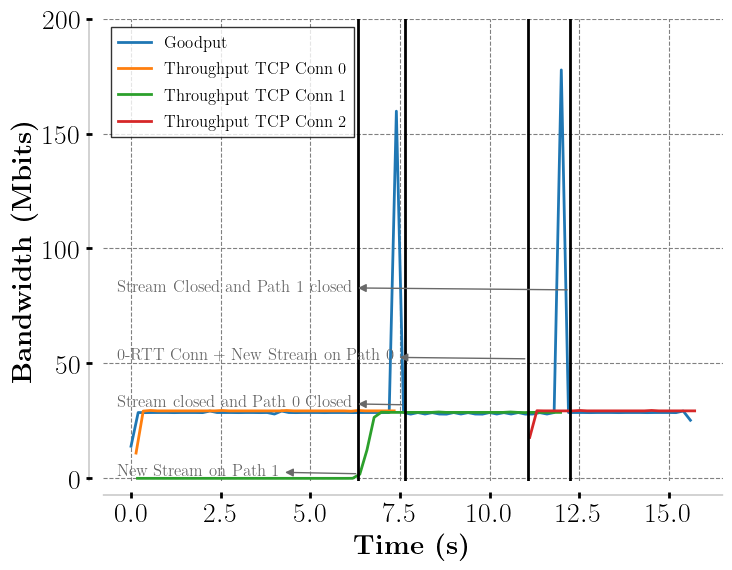
\includegraphics[scale=0.5]{figures/migration.png}
  \caption{Application-level connection migration during a 60MB file download}
  \label{fig:conn_migration}
\end{figure}
